% Compact PGFPlots panel for sampled surface11 BSC bit-scale decomposition.
% Requires \usepackage{pgfplots} and \pgfplotsset{compat=1.18}.
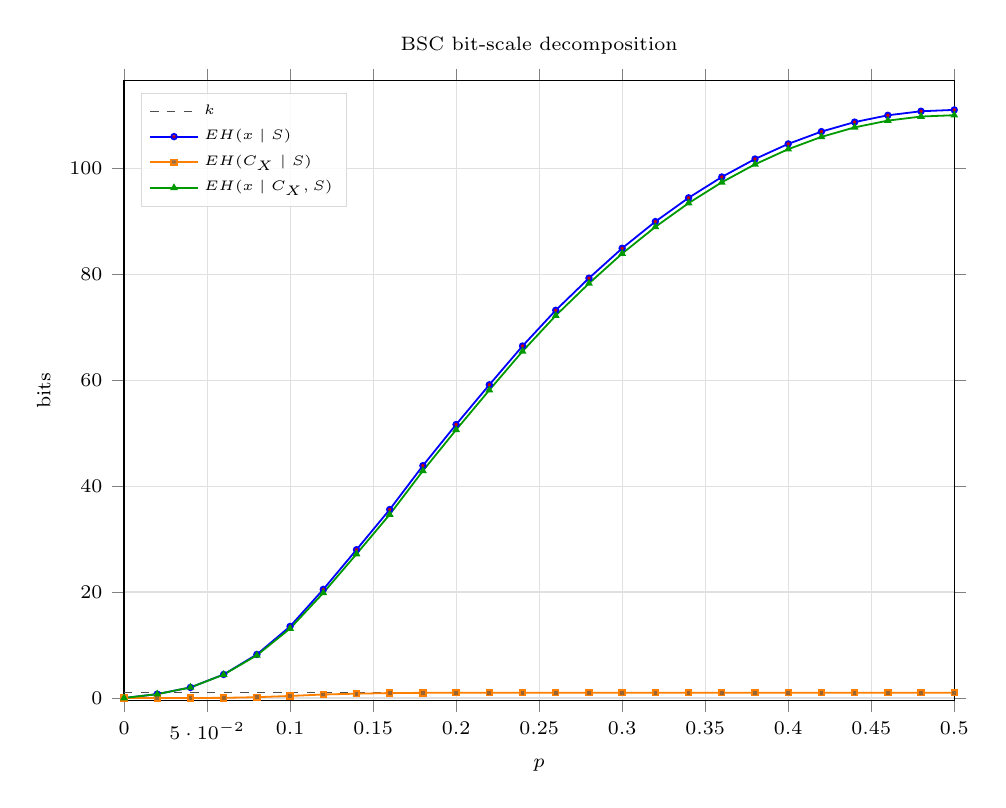
\begin{tikzpicture}
\begin{axis}[
  name=surface11BSCBitScaleAxis,
  width=\linewidth,
  height=0.78\linewidth,
  title={BSC bit-scale decomposition},
  title style={font=\scriptsize},
  xlabel={$p$},
  ylabel={bits},
  xmin=0, xmax=0.5,
  ymin=-0.5, ymax=116.55,
  grid=both,
  major grid style={black!12},
  minor grid style={black!6},
  tick align=outside,
  tick label style={font=\scriptsize},
  label style={font=\scriptsize},
  legend cell align={left},
  legend style={draw=black!15, fill=white, fill opacity=0.82, text opacity=1, at={(0.02,0.98)}, anchor=north west, font=\tiny},
]
\addplot[black!70, dashed, line width=0.55pt] coordinates {(0,1) (0.5,1)};
\addlegendentry{$k$}
\addplot+[color=blue, mark=*, mark size=1.0pt, line width=0.65pt]
coordinates {(0,0) (0.02,0.734688990658) (0.04,1.99831203137) (0.06,4.44692704397) (0.08,8.22288890142) (0.1,13.5074875114) (0.12,20.5000587691) (0.14,27.9924830997) (0.16,35.5719303002) (0.18,43.8565217947) (0.2,51.6202782147) (0.22,59.1146661146) (0.24,66.4396270333) (0.26,73.1814902563) (0.28,79.2425498427) (0.3,84.882400527) (0.32,89.9202253396) (0.34,94.4053248016) (0.36,98.3372640077) (0.38,101.729268648) (0.4,104.580921018) (0.42,106.902458539) (0.44,108.699263156) (0.46,109.978665613) (0.48,110.744874631) (0.5,111)};
\addlegendentry{$\mathbb{E}H(x\mid S)$}
\addplot+[color=orange, mark=square*, mark size=1.0pt, line width=0.65pt]
coordinates {(0,0) (0.02,0.00570634906307) (0.04,0.00462353912555) (0.06,0.032956023151) (0.08,0.157329679071) (0.1,0.388254826899) (0.12,0.663328665925) (0.14,0.818675911276) (0.16,0.9367477817) (0.18,0.977001917946) (0.2,1.00132971209) (0.22,0.998548032862) (0.24,1.00045900588) (0.26,0.999481886583) (0.28,0.999994430108) (0.3,0.999961697838) (0.32,1.000007331) (0.34,1.00000060875) (0.36,0.999999958785) (0.38,1.00000003951) (0.4,0.999999996537) (0.42,0.999999999852) (0.44,0.999999999992) (0.46,1) (0.48,1) (0.5,1)};
\addlegendentry{$\mathbb{E}H(C_X\mid S)$}
\addplot+[color=green!60!black, mark=triangle*, mark size=1.0pt, line width=0.65pt]
coordinates {(0,0) (0.02,0.728982641595) (0.04,1.99368849224) (0.06,4.41397102082) (0.08,8.06555922235) (0.1,13.1192326845) (0.12,19.8367301031) (0.14,27.1738071884) (0.16,34.6351825185) (0.18,42.8795198768) (0.2,50.6189485026) (0.22,58.1161180818) (0.24,65.4391680275) (0.26,72.1820083697) (0.28,78.2425554126) (0.3,83.8824388292) (0.32,88.9202180086) (0.34,93.4053241929) (0.36,97.3372640489) (0.38,100.729268609) (0.4,103.580921021) (0.42,105.902458539) (0.44,107.699263156) (0.46,108.978665613) (0.48,109.744874631) (0.5,110)};
\addlegendentry{$\mathbb{E}H(x\mid C_X,S)$}
\end{axis}
\end{tikzpicture}
